\documentclass{article}
\setlength{\parskip}{5pt} % esp. entre párrafos
\setlength{\parindent}{0pt} % esp. al inicio de un párrafo
\usepackage{amsmath} % mates
\usepackage{url} % que las URLs se vean lindos
\usepackage[top=25mm,left=20mm,right=20mm,bottom=25mm]{geometry} % márgenes
\usepackage{parskip}
\usepackage[utf8]{inputenc}
\usepackage[margin=1in]{geometry}
\usepackage{amsmath,amsfonts,amssymb,mathtools}
\usepackage{graphicx,float}
\usepackage{algorithmic}
\usepackage{minted}
\usepackage{subcaption}
\usepackage{multicol}
\usepackage{listings}
\usepackage{xcolor}
\usepackage[sort&compress,numbers]{natbib} % referencias
\usepackage{minted}
\usepackage{hyperref} % ligas de URLs
\usepackage{graphicx} % poner figuras
\usepackage[spanish]{babel} % otros idiomas
\usepackage{listings}
\author{Raul L.} % author
\title{Pr\'{a}ctica 7:Búsqueda local} %título
\date{\today}
\begin{document} % inicia contenido

\maketitle % cabecera


\section{Introducci\'{o}n}\label{intro} % sección y etiqueta
En la séptima práctica implementamos una optimización heurística sencilla para encontrar máximos locales de funciones, los ejemplos siendo de Womersley \citep{1} — los matemáticamente inclinados pueden consultar su trabajo por métodos de búsqueda más sofisticados, guiados por métodos matemáticos de mayor rigor \citep{2}.
\newline



Buscamos minimizar la función unidimensional, a partir de un punto seleccionado al azar, realizando movimientos locales. Estando en $x$, seleccionará al azar un $\varDelta x>0$ pequeño, calculará los valores $f( (x \pm \varDelta x)$ y seleccionará el menor de los dos como el siguiente valor de $x$. Esto se repite $k$ veces y aquel $x$ que produjo el menor valor de $f(x)$ se regresa como el resultado. Se realizarán $n$ réplicas, y el menor de ellos es el resultado de la búsqueda en sí. La primera versión es sencilla, ineficiente y con una sola réplica para poder entender el comportamiento de la búsqueda y visualizarla.

\section{Objetivo}
La tarea se trata de maximizar algún variante de la función bidimensional ejemplo, $g(x,y)$, con restricciones tipo $ - 3 \leq x $,y $ \leq 3 $, con la misma técnica del ejemplo unidimensional. La posición actual es un par $x,y$ y se ocupan dos movimientos aleatorios, $ \varDelta x$  y $\varDelta y $, cuyas combinaciones posibles proveen ocho posiciones vecino, de los cuales aquella que logra el mayor valor para g es seleccionado. Dibujado en tres dimensiones, $g(x,y)$ se ve así:\citep{2}.

\section{C\'{o}digo}
Para este código se utilizó como base el código de la doctora donde se hicieron modificaciones variando la función y los parámetros base como también se crearon los 5 puntos al mismo tiempo y se revisó con una $x$ el mejor valor conocido.

 Código en Python 

\url{https://satuelisa.github.io/simulation/p7.html}

{\bf Código creado en Python}

\url{https://github.com/Raullr28/Resultados/blob/main/P7/practica_7.py}

\renewcommand{\listingscaption}{Código}

\begin{listing}[H]
\begin{minted}{python}
def g(x, y):
    return np.exp(-x**2)+ np.exp(-y**2)

low = -6
high = -low
step = 0.20
tmax = 500

x = np.arange(low, high, step)
y = np.arange(low, high, step)
x, y = np.meshgrid(x, y)
z =np.exp(-x**2)+ np.exp(-y**2)

fig = plt.figure()
ax = plt.axes(projection='3d')
s = ax.plot_surface(x, y, z, cmap=cm.coolwarm, linewidth=0, antialiased=False)
ax.zaxis.set_major_locator(LinearLocator(10))
ax.zaxis.set_major_formatter(FormatStrFormatter('%.01f'))
fig.colorbar(s, shrink=0.5, aspect=5)
plt.savefig("p7_3dinicial.png")
plt.show()


  \end{minted}
  \label{lst:fibo}
  \caption{Representación de la función y parámetros utilizados.}
  
  
\end{listing}
\renewcommand{\listingscaption}{Código}
\begin{listing}[H]

\begin{minted}{python}
 
 for iteracion in range(tmax):#entra a hacer ciclo de la particula
        #mueve particula en x+right  y x-left
        deltax = uniform(0, step/5)#movimiento en x 
        leftx = currx - deltax  
        leftx = low if leftx < low+step else leftx #asegurar que la particula esta dentro 
        rightx = currx + deltax 
        rightx = high if rightx > high-step else rightx
        
        deltay = uniform(0, step/5)
        lefty = curry - deltay  
        lefty = low if lefty < low+step else lefty  
        righty = curry + deltay  
        righty = high if righty > high-step else righty

        lista=[(leftx, righty),(currx, righty),(rightx, righty),(leftx, curry),(rightx, curry),(leftx, lefty),(currx, lefty),(rightx, lefty)]
        v1 = g(leftx, righty)#valores evaluados en g 
        v2 = g(currx, righty)
        v3 = g(rightx, righty)
        v4 = g(leftx, curry)
        v5 = g(rightx, curry)
        v6 = g(leftx, lefty)
        v7 = g(currx, lefty)
        v8 = g(rightx, lefty)
        vecinos=[v1, v2, v3, v4, v5, v6, v7, v8]
        vecino_mayor=vecinos.index(max(vecinos))# guarda la posicion del vecino mayor   
        [currx, curry]=lista[vecino_mayor]#actualiza particula en posicion nueva
        if g(currx, curry) > g(bestx, besty):#Actualiza si es una mejor posicion 
            [bestx, besty] = [currx, curry]
  \end{minted}
  \label{lst:fibo}
  \caption{Representación ciclo de la partícula.}
\end{listing}

% Computational Results
\section{Resultados}
En la figura principal se muestra la función en 3D creada, en las imágenes siguientes se muestra el comportamiento de los 5 puntos al mismo tiempo marcando con una $x$ el mejor valor en el transcurso de las 500 repeticiones modificándose cada vez que algún punto mejore su valor.
%%%%%%%%%%%%%%%%%%%%% imagen 1
\begin{figure}[H]
\centering
\begin{subfigure}[b]{1.0\linewidth}
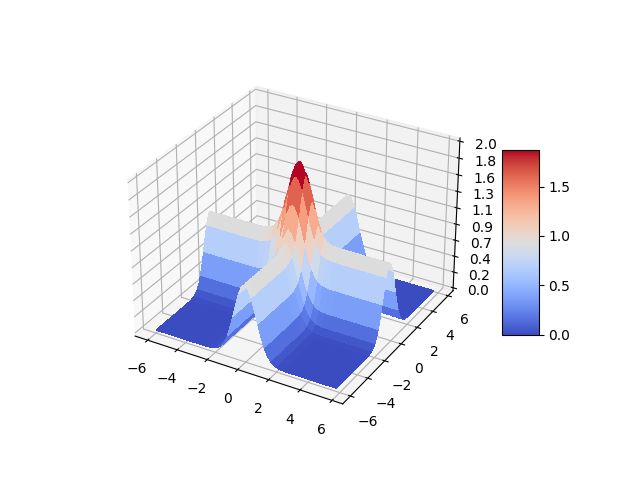
\includegraphics[width=\linewidth]{Imagen/p7_3dinicial.png}
\end{subfigure}
\caption{función 3D.}
\label{fig:westminster}
\end{figure}
%%%%%%%%%%%%%%%%%%%%%%%  final 

%%%%%%%%%%%%%%%%%%%%% imagen 2 y 3 
\begin{figure}[H]
\centering
\begin{subfigure}[Absoluto]{0.45\linewidth}
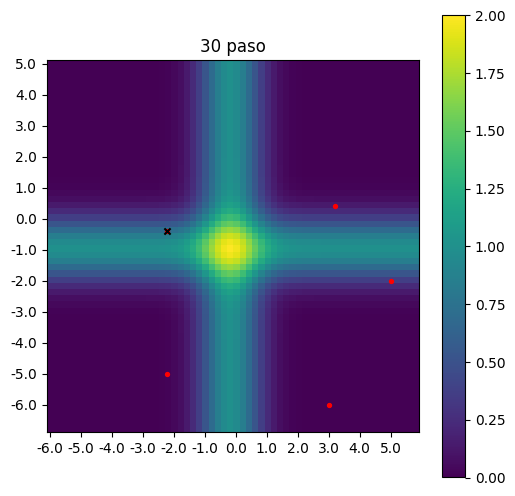
\includegraphics[width=\linewidth]{Imagen/p7p_29.png}
\caption{Paso 29 }
\end{subfigure}
\begin{subfigure}[Cuadrado]{0.45\linewidth}
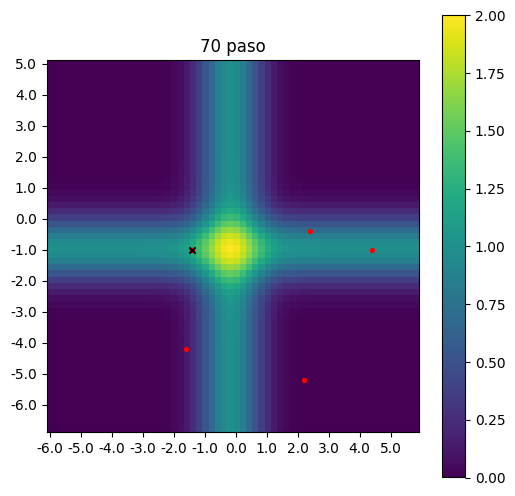
\includegraphics[width=\linewidth]{Imagen/p7p_69.png}
\caption{Paso 69}
\end{subfigure}
\caption{Comportamiento de el mejor punto.}
\label{fig:westminster}
\end{figure}
%%%%%%%%%%%%%%%%%%%%%%%  final 

%%%%%%%%%%%%%%%%%%%%% imagen 4 y 5
\begin{figure}[H]
\centering
\begin{subfigure}[Absoluto]{0.45\linewidth}
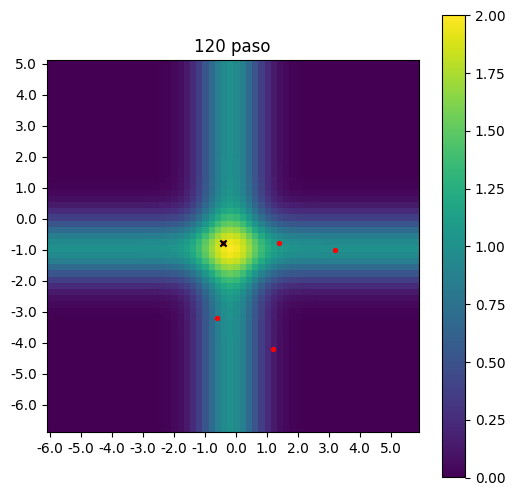
\includegraphics[width=\linewidth]{Imagen/p7p_119.png}
\caption{Paso 119}
\end{subfigure}
\begin{subfigure}[Cuadrado]{0.45\linewidth}
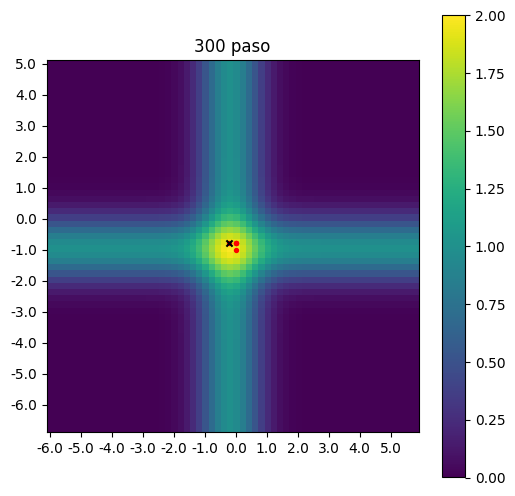
\includegraphics[width=\linewidth]{Imagen/p7p_299.png}
\caption{Paso 299}
\end{subfigure}
\caption{Comportamiento de el mejor punto.}
\label{fig:westminster}
\end{figure}
%%%%%%%%%%%%%%%%%%%%%%%  final 

\newpage
\section{Reto 1}
El primer reto es cambiar la regla del movimiento de una solución $x$ (un vector de dimensión arbitraria) a la siguiente a la de recocido simulado: para optimizar una función $f(x)$, se genera para la solución actual $x$ un sólo vecino $x$=$x + \varDelta x$ (algún desplazamiento local). Se calcula $ \delta =f(x\:') $$-$$ f(x)$ (para minimizar; maximizando la resta se hace al revés). Si $ \delta >0$, siempre se acepta al vecino $x\:'$como la solución actual ya que representa una mejora. Si $\delta<0$
, se acepta a $x\:'$ con probabilidad  
$exp( \delta / T)$ y rechaza en otro caso. Aquí $T$ es una temperatura que decrece en aquellos pasos donde se acepta una empeora; la reducción se logra multiplicando el valor actual de $T$ con $\xi < 1$, como por ejemplo $ 0.995$. Examina los efectos estadísticos del valor inicial de $T$ y el valor de $\xi$ en la calidad de la solución, es decir, qué tan bajo (para minimizar; alto para maximizar) el mejor valor termina siendo.

 %%%%%%%%%%%%%%%%%%%%% imagen 6
\begin{figure}[H]
\centering
\begin{subfigure}[b]{1.0\linewidth}
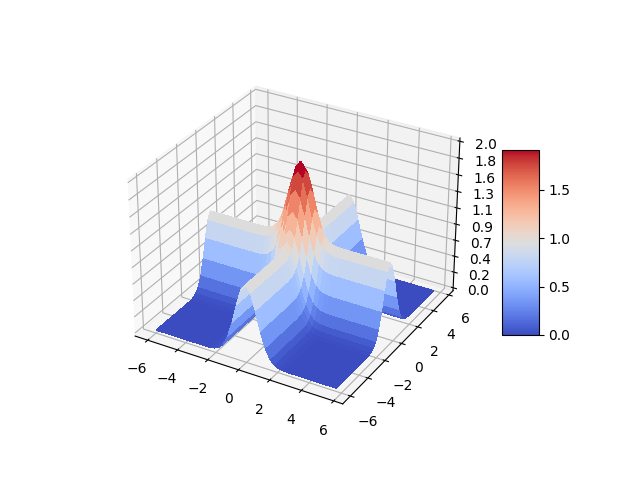
\includegraphics[width=\linewidth]{Imagen/Figure_1_r1.png}
\end{subfigure}
\caption{función 3D.}
\label{fig:westminster}
\end{figure}
%%%%%%%%%%%%%%%%%%%%%%%  final 
\section{Resultados}
 %%%%%%%%%%%%%%%%%%%%% imagen 7 y 8
\begin{figure}[H]
\centering
\begin{subfigure}[b]{0.45\linewidth}
\includegraphics[width=\linewidth]{Imagen/r7p_49.png}
\caption{Paso 50}
\end{subfigure}
\begin{subfigure}[b]{0.45\linewidth}
\includegraphics[width=\linewidth]{Imagen/r7p_499.png}
\caption{Paso 500}
\end{subfigure}
\caption{Comportamiento de el mejor punto.}
\label{fig:westminster}
\end{figure}
 %%%%%%%%%%%%%%%%%%%%% 
  %%%%%%%%%%%%%%%%%%%%% imagen 9 y 10
  \begin{figure}[H]
\centering
\begin{subfigure}[b]{0.45\linewidth}
\includegraphics[width=\linewidth]{Imagen/r7p_749.png}
\caption{Paso 750}
\end{subfigure}
\begin{subfigure}[b]{0.45\linewidth}
\includegraphics[width=\linewidth]{Imagen/r7p_999.png}
\caption{Paso1000}
\end{subfigure}
\caption{Comportamiento de el mejor punto.}
\label{fig:westminster}
\end{figure}
 %%%%%%%%%%%%%%%%%%%%% 
\newpage
 \section{Conclusión}

Se demostró que en la tarea base le costo menos a los puntos maximizar las posiciones de los puntos para poder encontrar el mejor lugar mientras que en el reto 1 les costo más.

 \bibliography{bibliografia.bib}
 \bibliographystyle{unsrtnat}

 \end{document}


